\newcommand{\invariantReprComparison}
{
\begin{figure}[t]
\centering
\begin{tikzpicture}[scale=1.5]
% \draw[draw=black, rounded corners=20pt] (0,0) rectangle (5,3);
\draw[draw=red, rounded corners=38pt] (0.5,0.25) rectangle (4,2.75);
\draw[draw=red, rounded corners=15pt] (1, 0.9) rectangle (3.2,2.1);

\draw[draw=blue, rounded corners=15pt, dash pattern={on 4.5pt off 4.5pt}] (2.3,0.9) rectangle (5,2.1);

\draw (1.2,0.3) node [anchor=south west][inner sep=0.75pt]   [align=left]{\tiny \textsc{SizeElem}};
% \draw (1.3,1) node [anchor=south west][inner sep=0.75pt]   [align=left]{\tiny \textsc{Elem}};
\draw (4.9,1) node [anchor=south east][inner sep=0.75pt]   [align=right]{\tiny \textsc{Reg}};
\draw (1.3,1) node [anchor=south west][inner sep=0.75pt]   [align=left]{\tiny \textsc{Elem}};

\draw (3.3,1.4) node [anchor=south west][inner sep=0.75pt]   [align=left]{\tiny \textit{Even}};
\draw (4.1,1.4) node [anchor=south west][inner sep=0.75pt]   [align=left]{\tiny \textit{EvenLeft}};
\draw (0.6,1.4) node [anchor=south west][inner sep=0.75pt]   [align=left]{\tiny \textit{LtLt}};
\draw (1.6,1.4) node [anchor=south west][inner sep=0.75pt]   [align=left]{\tiny \textit{Eq}};


\onslide<2->{\draw[draw=blue, rounded corners=55pt] (0,0.5) rectangle (6,3)};
% \draw[draw=black] (3,1) circle;
%\onslide<2->{\filldraw[black] (3,0.15) circle (2pt) node[anchor=west]{\small \textit{LtAsymmetric}}};
\onslide<3->{ \draw (4.5,2.75) node [anchor=south west][inner sep=0.75pt]   [align=left]{\tiny \textsc{FCTTA}}};
\end{tikzpicture}
\captionsetup{justification=centering}
\caption*{Сравнение выразительной силы различных абстрактных доменов \onslide<1>{\texttt{ Источник: Ю. О. Костюков, Автоматический вывод регулярных инвариантов программ с алгебраическими типами данных}}}
\end{figure}


}

\newcommand{\treeView}{
    \begin{figure*}
    \centering
    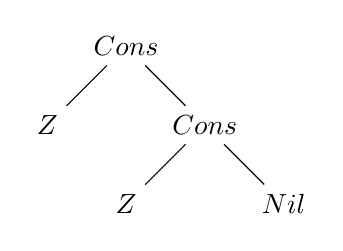
\begin{tikzpicture}[node distance=2cm,remember picture]
    
    
    \node (D) at (6,0) {$Cons$};
    \node (E) at (7,-1){$Cons$};
    \node (F) at (5,-1){$Z$};
    \node (F2) at (6,-2){$Z$};
    \node (F3) at (8,-2){$Nil$};
    \draw[-] (D) -- (E);
    \draw[-] (D) -- (F);
    \draw[-] (E) -- (F2);
    \draw[-] (E) -- (F3);
    
    
    \end{tikzpicture}
    \end{figure*}
    }


\newcommand{\StandartSync}{
    \begin{figure*}
    \centering
    \begin{tikzpicture}[node distance=2cm,remember picture, scale=0.8]
    
    \node (A) at (1,0) {$f$};
    \node (B) at (0,-1){$g$};
    \node (B1) at (0,-2){$a$};
    
    \node (C) at (2,-1){$g$};
    \node (C1) at (2,-2){$a$};
    \node (C2) at (3,-1){$\bigoplus$};
    
    \draw[-] (A) -- (B);
    \draw[-] (A) -- (C);
    \draw[-] (B) -- (B1);
    \draw[-] (C) -- (C1);
    
    \node (D) at (6,0) {$f$};
    \node (E) at (7,-1){$a$};
    \node (F) at (5,-1){$f$};
    \node (F1) at (4,-2){$a$};
    \node (F2) at (6,-2){$a$};
    
    \draw[-] (D) -- (E);
    \draw[-] (D) -- (F);
    \draw[-] (F) -- (F1);
    \draw[-] (F) -- (F2);
    
    \node (S1) at (8,-1){};
    \node (S2) at (9.5,-1){};
    \draw[->] (S1) -- (S2);
    
    
    \node (G) at (12,0) {$ff$};
    \node (H) at (11,-1){$fg$};
    \node (H1) at (10,-2){$aa$};
    \node (H2) at (12,-2){$\bot{}a$};
    \node (I) at (13,-1){$ga$};
    \node (I1) at (13,-2){$a\bot$};
    
    \draw[-] (G) -- (H);
    \draw[-] (H) -- (H1);
    \draw[-] (H) -- (H2);
    \draw[-] (G) -- (I);
    \draw[-] (I) -- (I1);
    
    \end{tikzpicture}
    \caption{Стандартная синхронизация двух термов}
    \label{fig:ref-stdSync}
    \end{figure*}
    }

\newcommand{\FullSync}{
    \begin{figure*}
    \centering
    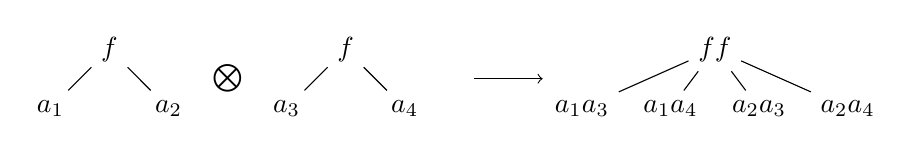
\begin{tikzpicture}[node distance=2cm,remember picture, scale=0.75]
    
    \node (A) at (1,0) {$f$};
    \node (B) at (0,-1){$a_1$};
    
    \node (C) at (2,-1){$a_2$};
    \node (C2) at (3,-0.5){$\bigotimes$};
    
    \draw[-] (A) -- (B);
    \draw[-] (A) -- (C);
    
    \node (D) at (5,0) {$f$};
    \node (E) at (6,-1){$a_4$};
    \node (F) at (4,-1){$a_3$};
    
    \draw[-] (D) -- (E);
    \draw[-] (D) -- (F);
    
    \node (S1) at (7,-0.5){};
    \node (S2) at (8.5,-0.5){};
    \draw[->] (S1) -- (S2);
    
    
    \node (G) at (11.25,0) {$ff$};
    \node (H) at (9,-1){$a_1a_3$};
    \node (H2) at (10.5,-1){$a_1a_4$};
    \node (H3) at (12,-1){$a_2a_3$};
    \node (I) at (13.5,-1){$a_2a_4$};
    
    \draw[-] (G) -- (H);
    \draw[-] (G) -- (I);
    \draw[-] (G) -- (H2);
    \draw[-] (G) -- (H3);

    
    \end{tikzpicture}
    \caption{Стандартная синхронизация двух термов}
    \label{fig:ref-stdSync}
    \end{figure*}
    }
    
    \newcommand{\ListLen}{
    \begin{figure*}
    \centering
    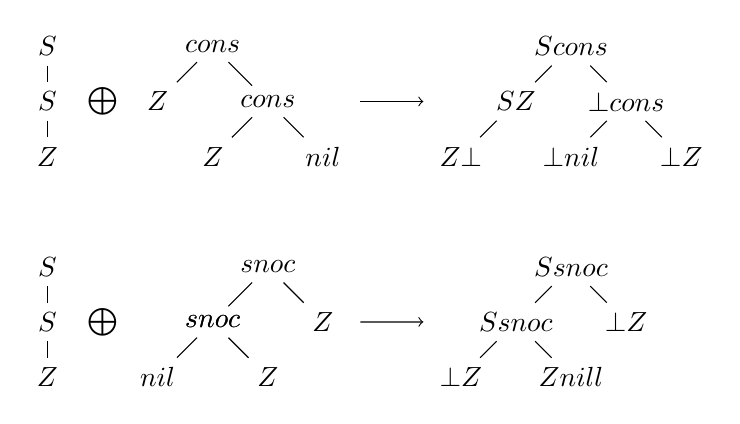
\begin{tikzpicture}[node distance=2cm,remember picture,scale=0.7]
    
    \node (A) at (0,0) {$S$};
    \node (B) at (0,-1){$S$};
    \node (B1) at (0,-2){$Z$};
    
    \draw[-] (A) -- (B);
    \draw[-] (B) -- (B1);
    
    
    \node (D) at (3,0) {$cons$};
    \node (E) at (4,-1){$cons$};
    \node (F) at (2,-1){$Z$};
    \node (E1) at (3,-2){$Z$};
    \node (E2) at (5,-2){$nil$};
    \node (E3) at (1,-1){$\bigoplus$};
    \draw[-] (D) -- (E);
    \draw[-] (D) -- (F);
    \draw[-] (E) -- (E1);
    \draw[-] (E) -- (E2);
    
    \node (S1) at (5.5,-1){};
    \node (S2) at (7,-1){};
    \draw[->] (S1) -- (S2);
    
    
    \node (G) at (9.5,0) {$Scons$};
    \node (H) at (8.5,-1){$SZ$};
    \node (H1) at (7.5,-2){$Z\bot$};
    \node (I) at (10.5,-1){$\bot{}cons$};
    \node (I1) at (11.5,-2){$\bot{}Z$};
    \node (I2) at (9.5,-2){$\bot{}nil$};
    
    \draw[-] (G) -- (H);
    \draw[-] (H) -- (H1);
    \draw[-] (G) -- (I);
    \draw[-] (I) -- (I1);
    \draw[-] (I) -- (I2);
    
    % \node (TextA) at (5.75,-3){(а) стандартная синхронизация};
    
    
    
    \node (J) at (0,-4) {$S$};
    \node (K) at (0,-5){$S$};
    \node (K1) at (0,-6){$Z$};
    
    \draw[-] (J) -- (K);
    \draw[-] (K) -- (K1);
    
    
    \node (L) at (4,-4) {$snoc$};
    \node (M) at (5,-5){$Z$};
    \node (N) at (3,-5){$snoc$};
    \node (N) at (3,-5){$snoc$};
    \node (N1) at (2,-6){$nil$};
    \node (N2) at (4,-6){$Z$};
    \node (N3) at (1,-5){$\bigoplus$};
    \draw[-] (L) -- (M);
    \draw[-] (L) -- (N);
    \draw[-] (N) -- (N1);
    \draw[-] (N) -- (N2);
    
    \node (S11) at (5.5,-5){};
    \node (S22) at (7,-5){};
    \draw[->] (S11) -- (S22);
    
    \node (N) at (9.5,-4) {$Ssnoc$};
    \node (O) at (8.5,-5){$Ssnoc$};
    \node (P) at (10.5,-5){$\bot{}Z$};
    \node (O1) at (9.5,-6){$Znill$};
    \node (O2) at (7.5,-6){$\bot{}Z$};
    
    \draw[-] (N) -- (O);
    \draw[-] (N) -- (P);
    \draw[-] (O) -- (O1);
    \draw[-] (O) -- (O2);
    
    % \node (TextB) at (5.75,-7){(б) нестандартная синхронизация};
    
    \end{tikzpicture}
    \caption{Варианты синхронизации числа Пеано и списка}
    \label{fig:ref-listLen}
    \end{figure*}
    }
    
    \newcommand{\eqAutomata}{
    \begin{figure*}[h]
    \centering
    \begin{tikzpicture}[node distance=2cm,remember picture]
    \draw (-1.5,-1.5) -- (-2, -0.5) -- (-1.5,0.5);
    
    \node (A) at (0,0) {$g$};
    \node (A1) at (-1,-1){$t_1$};
    \node (A2) at (0,-1){$\dots$};
    \node (A2) at (1,-1){$t_n$};
    \draw[-] (A) -- (A1);
    \draw[-] (A) -- (A2);
    \node (D) at (1.5,-0.5) {$,$};
    
    \node (B) at (3,0) {$\bot$};
    \node (B1) at (2,-1) {$t_1$};
    \node (B2) at (3,-1) {$\dots$};
    \node (B3) at (4,-1) {$\bot$};
    \draw[-] (B) -- (B1);
    \draw[-] (B) -- (B3);
    
    \node (dots) at (5,-0.5) {$,\dots,$};
    
    \node (C) at (7,0) {$\bot$};
    \node (C1) at (6,-1) {$\bot$};
    \node (C2) at (7,-1) {$\dots$};
    \node (C3) at (8,-1) {$t_n$};
    \draw[-] (C) -- (C1);
    \draw[-] (C) -- (C3);
    
    \draw (8.5,-1.5) -- (9, -0.5) -- (8.5,0.5);
    
    \end{tikzpicture}
    \label{fig:ref-listLen}
    \end{figure*}
    }
    
    \newcommand{\eqInduction}{
    \begin{figure*}[h]
    \centering
    \begin{tikzpicture}[node distance=2cm,remember picture]
    
    
    \node (A) at (-1.5,0) {$g$};
    \node (A1) at (-2.5,-1){$f_1$};
    \node (A2) at (-1.5,-1){$\dots$};
    \node (A2) at (-0.5,-1){$f_n$};
    
    \node (E1) at (-3,-2.25){$t^1_1$};
    \node (E12) at (-2.5,-2.25){$\dots$};
    \node (E2) at (-2,-2.25){$t^1_n$};
    \node (E3) at (-1,-2.25){$t^n_1$};
    \node (E34) at (-0.5,-2.25){$\dots$};
    \node (E4) at (0,-2.25){$t^n_n$};
    
    \draw[-] (A) -- (A1);
    \draw[-] (A) -- (A2);
    \draw[-] (A1) -- (E1);
    \draw[-] (A1) -- (E2);
    \draw[-] (A2) -- (E3);
    
    \draw[-] (A2) -- (E4);
    
    
    \node (D) at (0.5,-1.25) {$,$};
    
    \node (B) at (3,0) {$\bot$};
    \node (B1) at (2,-1) {$f_1$};
    \node (B2) at (3,-1) {$\dots$};
    \node (B3) at (4,-1) {$\bot$};
    \node (E1) at (1.5,-2.25) {$t^1_1$};
    \node (E2) at (2,-2.25) {$\dots$};
    \node (E3) at (2.5,-2.25) {$t^1_n$};
    
    \draw[-] (B) -- (B1);
    \draw[-] (B) -- (B3);
    \draw[-] (B1) -- (E1);
    \draw[-] (B1) -- (E3);
    
    \node (dots) at (5,-1.25) {$,\dots,$};
    
    \node (C) at (7,0) {$\bot$};
    \node (C1) at (6,-1) {$\bot$};
    \node (C2) at (7,-1) {$\dots$};
    \node (C3) at (8,-1) {$f_n$};
    \node (D1) at (7.5, -2.5) {$t^n_1$};
    \node (D2) at (8, -2.5) {$\dots$};
    \node (D3) at (8.5, -2.5) {$t^n_n$};
    \draw[-] (C) -- (C1);
    \draw[-] (C) -- (C3);
    \draw[-] (C3) -- (D1);
    \draw[-] (C3) -- (D3);

    \end{tikzpicture}
    \label{fig:ref-listLen}
    \end{figure*}
    }
    
    \newcommand{\PattternAutomata}{
    \begin{figure*}
    \centering
    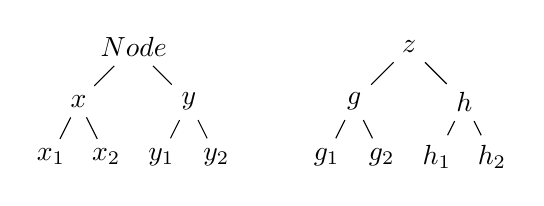
\begin{tikzpicture}[node distance=2cm,remember picture,scale=0.7]
    
    \node (A) at (1,0) {$Node$};
    \node (B) at (0,-1){$x$};
    \node (B1) at (-0.5,-2){$x_1$};
    \node (B2) at (0.5,-2){$x_2$};
    
    \node (C) at (2,-1){$y$};
    \node (C1) at (1.5,-2){$y_1$};
    \node (C2) at (2.5,-2){$y_2$};
    
    \draw[-] (A) -- (B);
    \draw[-] (A) -- (C);
    \draw[-] (B) -- (B1);
    \draw[-] (B) -- (B2);
    
    \draw[-] (C) -- (C1);
    \draw[-] (C) -- (C2);
    
    \node (D) at (6,0) {$z$};
    \node (E) at (5,-1){$g$};
    \node (F) at (7,-1){$h$};
    \node (E1) at (4.5,-2){$g_1$};
    \node (E2) at (5.5,-2){$g_2$};
    
    \node (F1) at (6.5,-2){$h_1$};
    \node (F2) at (7.5,-2){$h_2$};
    
    \draw[-] (D) -- (E);
    \draw[-] (D) -- (F);
    \draw[-] (E) -- (E1);
    \draw[-] (E) -- (E2);
    \draw[-] (F) -- (F1);
    \draw[-] (F) -- (F2);
    
    \end{tikzpicture}
    \label{fig:ref-stdSync}
    \end{figure*}
    }
% \newcommand{\invariantReprComparison}
% {
% \begin{figure}[t]
% \tikzset{every picture/.style={line width=0.75pt}} %set default line width to 0.75pt        
% \centering
% \begin{tikzpicture}[x=0.75pt,y=0.75pt,yscale=-0.35,xscale=0.45,every node/.style={scale=0.65}]
% %uncomment if require: \path (0,300); %set diagram left start at 0, and has height of 300

% % Big red one
% \draw  [color={rgb, 255:red, 208; green, 2; blue, 27 }  ,draw opacity=1 ] (135.1,92.13) -- (400.9,92.13) .. controls (434.08,92.13) and (454.5,132.64) .. (454.5,182.63) .. controls (454.5,232.61) and (434.08,273.13) .. (400.9,273.13) -- (135.1,273.13) .. controls (109.92,273.13) and (89.5,232.61) .. (89.5,182.63) .. controls (89.5,132.64) and (109.92,92.13) .. (135.1,92.13) -- cycle ;
% % Right blue
% \draw  [color={rgb, 255:red, 144; green, 19; blue, 254 }  ,draw opacity=1 ][dash pattern={on 4.5pt off 4.5pt}] (255.92,124.77) -- (357.58,124.77) .. controls (370.79,124.77) and (381.5,150.68) .. (381.5,182.63) .. controls (381.5,214.57) and (370.79,240.48) .. (357.58,240.48) -- (255.92,240.48) .. controls (242.71,240.48) and (232,214.57) .. (232,182.63) .. controls (232,150.68) and (242.71,124.77) .. (255.92,124.77) -- cycle ;
% % \draw  [color={rgb, 255:red, 144; green, 19; blue, 254 }  ,draw opacity=1 ][dash pattern={on 4.5pt off 4.5pt}] (295.12,92.12) -- (423.38,92.12) .. controls (458.24,92.12) and (486.5,132.64) .. (486.5,182.63) .. controls (486.5,232.61) and (458.24,273.13) .. (423.38,273.13) -- (295.12,273.13) .. controls (260.26,273.13) and (232,232.61) .. (232,182.63) .. controls (232,132.64) and (260.26,92.12) .. (295.12,92.12) -- cycle ;
% % Small left red
% \draw  [color={rgb, 255:red, 208; green, 2; blue, 27 }  ,draw opacity=1 ] (185.92,124.77) -- (287.58,124.77) .. controls (300.79,124.77) and (311.5,150.68) .. (311.5,182.63) .. controls (311.5,214.57) and (300.79,240.48) .. (287.58,240.48) -- (185.92,240.48) .. controls (172.71,240.48) and (162,214.57) .. (162,182.63) .. controls (162,150.68) and (172.71,124.77) .. (185.92,124.77) -- cycle ;

% % Text Node
% \draw (115,248) node [anchor=north west][inner sep=0.75pt]   [align=left]
% % {\hyperref[sec:sizeelem-def]{$\sizeelemclass$}};
% {$\regelemclass$};
% % Text Node
% \draw (175,213) node [anchor=north west][inner sep=0.75pt]   [align=left]
% % {\hyperref[defn:elemclass]{$\elemclass$}};
% {$\elemclass$};
% % Text Node
% \draw (330,213) node [anchor=north west][inner sep=0.75pt]   [align=left]
% % {\hyperref[defn:regelemclass]{$\regelemclass$}};
% {$\regclass$};
% % Text Node
% % \draw (415,217) node [anchor=north west][inner sep=0.75pt]   [align=left]
% % {\hyperref[defn:regclass]{$\regclass$}};
% % {$\regclass$};
% \end{tikzpicture}
% \caption{Comparison of the expressive power of three abstract domains.}
% \label{fig:repr-comparison}
% \end{figure}
% }

\newcommand{\ltAutomaton}{
    \begin{figure*}
    \centering
    \begin{tikzpicture}[scale=0.7]
 
    \node [state] {$q_0$};
    \node (q0) [state,
    initial,
    initial left,
    initial distance=0.5cm,
    initial text=$\tuple{\bot, \bot}$
] {$q_0$};
    \node (q1) [state, accepting] at (3,1) {$q_1$};
    \node (q2) [state] at (3,-1) {$q_2$};

    \path [-stealth, thick]
        (q0) edge [bend left] node [above] {$\tuple{\bot, Z}$}   (q1)
        (q0) edge [bend right] node [below] {$\tuple{Z, \bot}$}   (q2)
        (q1) edge [loop right]  node {*}()
        (q2) edge [loop right]  node {*}();

    \end{tikzpicture}
    \end{figure*}
}

\newcommand{\evenAutomaton}{
    \begin{figure*}
    \centering
    \begin{tikzpicture}[scale=0.7]
 
    \node [state] {$q_0$};
    \node (q0) [state, accepting,
    initial,
    initial left,
    initial distance=0.5cm,
    initial text=$Z$
] {$q_0$};
    \node (q1) [state] at (3,0) {$q_1$};

    \path [-stealth, thick]
        (q0) edge [bend left] node [above] {$S$}   (q1)
        (q1) edge [bend left] node [below] {$S$}   (q0)

    \end{tikzpicture}
    \end{figure*}
}

\newcommand{\workflow}{
    \begin{figure*}
    \centering
    \begin{tikzpicture}[scale=1.07][thick]
    % \draw[draw=black] (1,0) rectangle (10,-3);
    % \node (1) [draw, rounded rectangle] at (2, -1) {rounded rectangle};
    
    \draw (1.1,-0.6) node [anchor=north west][inner sep=0.75pt]   [align=left]{\textsc{RInGen}};
    \draw[draw=black] (1,-0.5) rectangle (12,-2.5) ;
    
    \draw[draw=black, rounded corners] (2,-1) rectangle (6,-2) ;
    \draw (4,-1.5) node [inner sep=0.75pt] [align=center] {\small Условия верификации \\ \small над АТД};

    \draw[draw=black, rounded corners] (7,-1) rectangle (11,-2) ;
    \draw (9,-1.5) node [inner sep=0.75pt] [align=center] {\small Условия верификации \\ \small над EUF};  

 
    \draw[draw=black, rounded corners] (2.5,-3) rectangle (10.5,-6) ;
    \draw (6.5,-4.5) node [inner sep=0.75pt] [align=center]
    {\small Логическое представление автоматов \\ \\
    \small $\begin{aligned}
        S(x) &= y\\
        Q_\mathcal{B} &= \{Z, S\} \times Q\\
        F_\mathcal{B} &= \{ \langle S, q \rangle \ | q \in F_{=}\}\\
        \delta_\mathcal{B}(f, g, \langle g_1, q \rangle) &= \langle g, \delta_{=}(f, g_1, q) \rangle 
    \end{aligned}$};
    
    \draw[draw=black, rounded corners] (2.25,-6.5) rectangle (5.75,-7.5) ;
    \draw (4,-7) node [inner sep=0.75pt] [align=center] {\small Конечная модель};

    \draw[draw=black, rounded corners] (7.3,-6.5) rectangle (10.7,-7.5) ;
    \draw (9,-7) node [inner sep=0.75pt] [align=center] {\small Инвариант исходной\\ \small программы};
    
    \node[main node] (1) at (11, -1.5);
    \node (2) at (10.5,-4.5);
    \node (3) at (2.5,-4.5);
    \node (4) at (2.25,-7);
    \path[-stealth]
        (1.center) edge[bend left=60] (2.center)
        (3.center) edge[bend right=70] (4.center);

    \draw[-stealth] (6,-1.5) -- (7,-1.5);
    \draw[-stealth] (5.75,-7) -- (7.3,-7);
    \end{tikzpicture}
    \end{figure*}
}
